\documentclass{article}
% main document, called main.tex

\usepackage{tikz}
\usepackage{fullpage}
\usetikzlibrary{decorations.markings}

\tikzstyle{startstop} = [rectangle, rounded corners, text centered, draw=black]
\tikzstyle{arrow} = [thick,->,>=stealth]

\newcommand{\arrowIn}{
	\tikz \draw[-stealth,scale=1] (-1pt,0) -- (1pt,0);
}

\begin{document}	
\centering
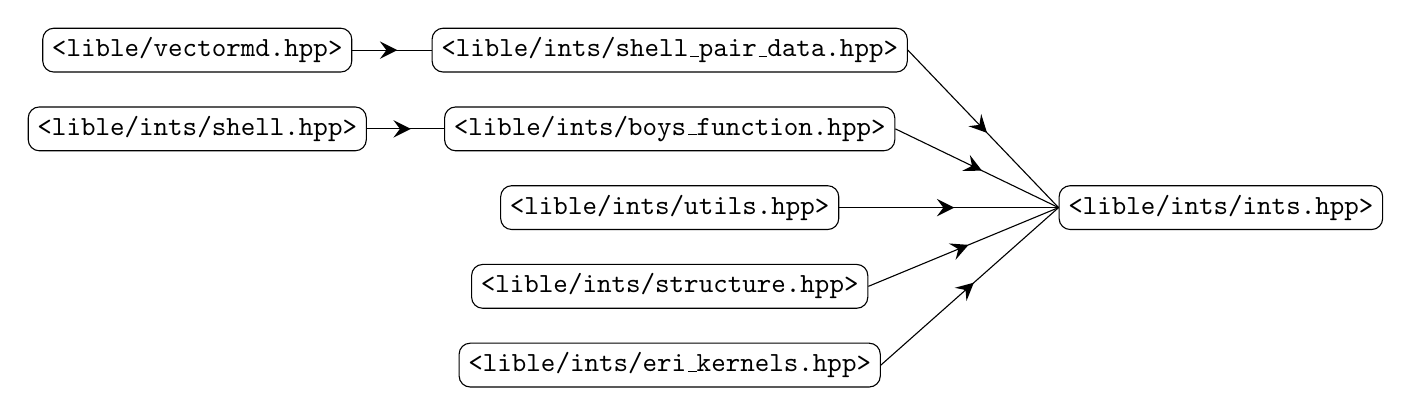
\begin{tikzpicture}
	\node (ints) at (12, 2)[startstop] {\texttt{<lible/ints/ints.hpp>}};
	\node (spdata) at (5, 4) [startstop] {\texttt{<lible/ints/shell\_pair\_data.hpp>}};
	\node (boysfun) at (5, 3) [startstop] {\texttt{<lible/ints/boys\_function.hpp>}};
	\node (utils) at (5, 2) [startstop] {\texttt{<lible/ints/utils.hpp>}};
	\node (structure) at (5, 1) [startstop] {\texttt{<lible/ints/structure.hpp>}};
	\node (erikernels) at (5, 0) [startstop] {\texttt{<lible/ints/eri\_kernels.hpp>}};	
	\node (vectormd) at (-1, 4) [startstop] {\texttt{<lible/vectormd.hpp>}};
	\node (shell) at (-1, 3) [startstop] {\texttt{<lible/ints/shell.hpp>}};				
		%\draw [arrow] (vectormd) -- (spdata);
		%\draw [arrow] (shell) -- (boysfun);
		%\draw [arrow] (spdata.east) -- (ints.west);
		%\draw [arrow] (boysfun.east) -- (ints.west);
		%\draw [arrow] (utils) -- (ints.west);
		%\draw [arrow] (structure.east) -- (ints.west);
		%\draw [arrow] (erikernels.east) -- (ints.west);
	\draw (vectormd.east) -- (spdata.west) node[sloped, pos=0.5, allow upside down, scale=2]{\arrowIn};
	\draw (shell.east) -- (boysfun.west) node[sloped, pos=0.5, allow upside down, scale=2]{\arrowIn};
	\draw (spdata.east) -- (ints.west) node[sloped, pos=0.5, allow upside down, scale=2]{\arrowIn};
	\draw (boysfun.east) -- (ints.west) node[sloped, pos=0.5, allow upside down, scale=2]{\arrowIn};
	\draw (utils.east) -- (ints.west) node[sloped, pos=0.5, allow upside down, scale=2]{\arrowIn};
	\draw (structure.east) -- (ints.west) node[sloped, pos=0.5, allow upside down, scale=2]{\arrowIn};
	\draw (erikernels.east) -- (ints.west) node[sloped, pos=0.5, allow upside down, scale=2]{\arrowIn};
\end{tikzpicture}
\newpage
\centering
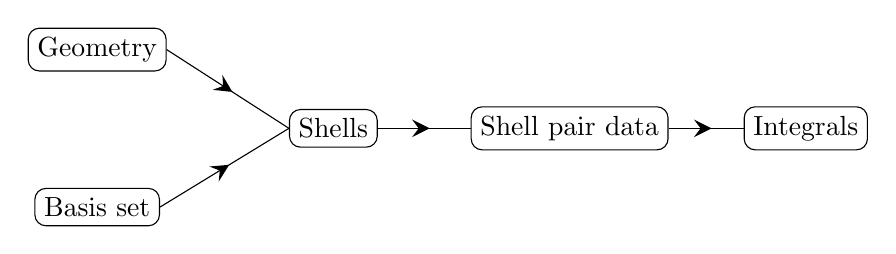
\begin{tikzpicture}
	\node (geom) at (-1, 2) [startstop] {Geometry};
	\node (basis) at (-1, 0) [startstop] {Basis set};
	\node (shells) at (2, 1) [startstop] {Shells};
	\node (spdata) at (5, 1) [startstop] {Shell pair data};
	\node (integrals) at (8, 1) [startstop] {Integrals};
	\draw (geom.east) -- (shells.west) node[sloped, pos=0.5, allow upside down, scale=2]{\arrowIn};
	\draw (basis.east) -- (shells.west) node[sloped, pos=0.5, allow upside down, scale=2]{\arrowIn};
	\draw (shells.east) -- (spdata.west) node[sloped, pos=0.5, allow upside down, scale=2]{\arrowIn};
	\draw (spdata.east) -- (integrals.west) node[sloped, pos=0.5, allow upside down, scale=2]{\arrowIn};
\end{tikzpicture}
\newpage
\centering
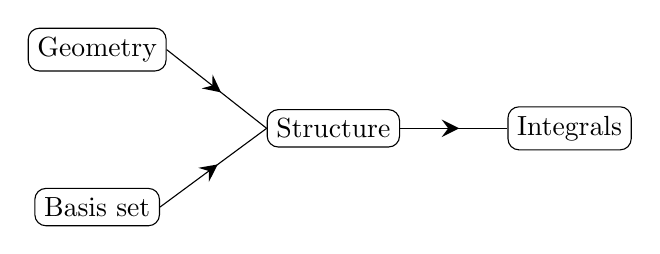
\begin{tikzpicture}
	\node (geom) at (-1, 2) [startstop] {Geometry};
	\node (basis) at (-1, 0) [startstop] {Basis set};
	\node (structure) at (2, 1) [startstop] {Structure};
	\node (integrals) at (5, 1) [startstop] {Integrals};
	\draw (geom.east) -- (structure.west) node[sloped, pos=0.5, allow upside down, scale=2]{\arrowIn};
	\draw (basis.east) -- (structure.west) node[sloped, pos=0.5, allow upside down, scale=2]{\arrowIn};	
	\draw (structure.east) -- (integrals.west) node[sloped, pos=0.5, allow upside down, scale=2]{\arrowIn};	
\end{tikzpicture}

\end{document}














